\documentclass[article]{moderncv}
\moderncvtheme[blue]{classic}
\usepackage[utf8]{inputenc}
\usepackage{amsmath}
\usepackage{amsfonts}
\usepackage{amssymb}
\usepackage{graphicx}
\usepackage{xcolor}
\usepackage{xpatch}
\PassOptionsToPackage{hidelinks, linkcolor=black}{hyperref}
\usepackage{geometry}
\geometry{
  hmargin=1cm,
  top=3mm,
  bottom=5mm
} 
\xpatchcmd\cventry{,}{}{}{}
\setlength{\parindent}{0pt}

\nopagenumbers{} 

\title{Sr. Embedded Linux Designer}
\firstname{}
\familyname{\\[0.5 cm]Anis CHALI}
\extrainfo{

\includegraphics[scale=0.25]{img/adr.png} \textcolor{black}{780 rue de Belmont, G1V2W9 Québec, QC}\\

\includegraphics[scale=0.2]{img/tel.png} \textcolor{black}{(+1) 581 997 9445}\\

\includegraphics[scale=0.2]{img/mail.png} \textcolor{black}{\emaillink{anis.chali1@outlook.com}}\\

\includegraphics[scale=0.015]{img/in.png} \href{https://www.linkedin.com/in/anis-chali-42564614a}{anischali}\\

\includegraphics[scale=0.008]{img/git.png} \href{https://www.github.com/anischali/}{anischali}\\
\textcolor{black}{Nationality: French}\\
\textcolor{black}{30 years old}
}
\photo[64pt][0.5pt]{img/ph2.jpeg}

\begin{document}
\maketitle

\section{Experience:}
\cventry{\newline{}
\includegraphics[height=30pt, width=55pt]{img/exfo.jpeg}}{Embedded Linux \& Microcontroller Designer}{\small{\newline{}February 2020 - today\newline{}Quebec, QC, Canada}}{}{}{}{}
\cventry{\newline{}
\includegraphics[height=25pt, width=55pt]{img/scc.jpeg}}{System technecian \& scripting}{\small{\newline{}August 2019 - December 2019\newline{}Paris, France}}{}{}{}{}
\cventry{\newline{}
\includegraphics[height=20pt, width=50pt]{img/p8.png}}{Internship in artificial Intelligence lab}{\small{\newline{}June 2019 - Jully 2019\newline{}Paris 8 UNiversity - Saint-Denis, Île-de-France, France}}{}{}{}{}
\cventry{\newline{}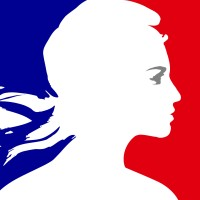
\includegraphics[height=30pt, width=30pt]{img/mj.jpeg}}{System technecian}{\small{\newline{}May 2018 - September 2018\newline{}Paris, France}}{}{}{}{}

\section{Education:}
\cventry{\newline{}
\includegraphics[height=20pt, width=50pt]{img/p8.png}}{Computer Science Bachelor}{\small{\newline{2015-2019}\newline{}Paris 8 UNiversity - Saint-Denis, Île-de-France, France}}{}{}{}
\section{Computer skills \& Languages:}
\subsection{Computer:}
\cventry{\newline{}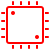
\includegraphics[height=18pt, width=20pt]{img/cpu.png}}{Embedded:}%
{Yocto, Linux kernel, DeviceTree, FreeRTOS, Zephyr, MCUXpresso, HID Over I2C, HID Over USB, U-boot, STM32, Smart Batteries, SD Card, Audio, Atmel SAM \& AVR, buildroot, cross compile, RaspberryPi, BananaPi, Logic Analyzers, JLink segger.}{}{}{}
\cventry{\newline{}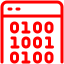
\includegraphics[height=18pt, width=20pt]{img/prog.png}}{Programming Languages:}%
{C/C++, Python, C\#, QT/Qml, Bash, PowerShell, Java, JS, SQL, CMake, Autotools, Makefile}{}{}{}
\cventry{\newline{}
\includegraphics[height=18pt, width=20pt]{img/tech.png}}{Technos:}%
{OpenSSL, WebRTC, P2P (lite-p2p: DTLS/TLS, STUN/TURN), NTP, DHCP, cryptsetup, flutter, secure boot, docker, GitHub, Gitlab, JIRA, Doxygen, \LaTeX, Azure, git, ostree OTA, OpenGL, repo, CI/CD, kas, west.}{}{}{}
\cventry{\newline{}
\includegraphics[height=18pt, width=20pt]{img/linux.png}}{Drivers:}%
{\textbf{Linux:} USB/USB Gadgets, HID Composite (power supply, rtc, i2c bridge, firmware, gpio, typec, led) , rfkill-gpio, sfp, drm, virtual keyboard. 
\textbf{Windows:} KMDF (USB, PCI)}{}{}{}
\cventry{\newline{}
\includegraphics[height=18pt, width=20pt]{img/tools.png}}{Tools:}%
{Linux Fedora/Ubuntu, NixOS, VSCode, Wireshark, Remmina, meld, qemu, nginx, wsl, Hyper-V, QtCreator, Atmel/Microchip Studio, EasyEDA, Mentor Graphics.}{}{}{}
\cventry{\newline{}
\includegraphics[height=18pt, width=20pt]{img/ai.png}}{Artificial Intelligence (coded in C/C++):}%
{\textbf{Unsupervised:} Self Organized Maps (SOM), Adaptive Resonance Theory (Art 2).  \textbf{Supervised:} Fuzzy ARTMap, Multi Layer Perceptron (MLP).}{}{}{}
\subsection{Languages:}
\cventry{
\includegraphics[height=18pt, width=20pt]{img/lang.png}}{}%
{\textbf{Kabyle, Arabic:} Native, \textbf{French:} Fluent, \textbf{English:} Professional}{}{}{}
\section{Hobbies:}
\cvline{}{Reading, Traveling, Chess game, Archery, Fishing, Electronic board design}
\end{document}